\chapter{Introduction}
\label{chap:introduction}
\pagenumbering{arabic}

%%%%%%%%%%%%%%%%%%%%%%%%%%%%%%%%%%%%%%%%%%%%%%%%%%%%%%%%%%%%%%%%%%%%%%%%%%%%%%%%%%%%%%%%%%%%%%%%%%%%

The objective of this project was to implement a control system for an existing hexapod-type robot (shown in \autoref{fig:hexapod}) through the use of the Robot Operating System (ROS) \cite{ros_site}. By attempting to implement a number of complex behaviours such as environment mapping and autonomous navigation, we aimed to evaluate the usefulness of ROS as a framework for rapidly developing these control systems. Specifically, we looked to explore a range of standard and community-provided packages available for use through ROS which provide state-of-the-art functionality, including those that were necessary for this control system.

\begin{figure}[t]
    \centering
    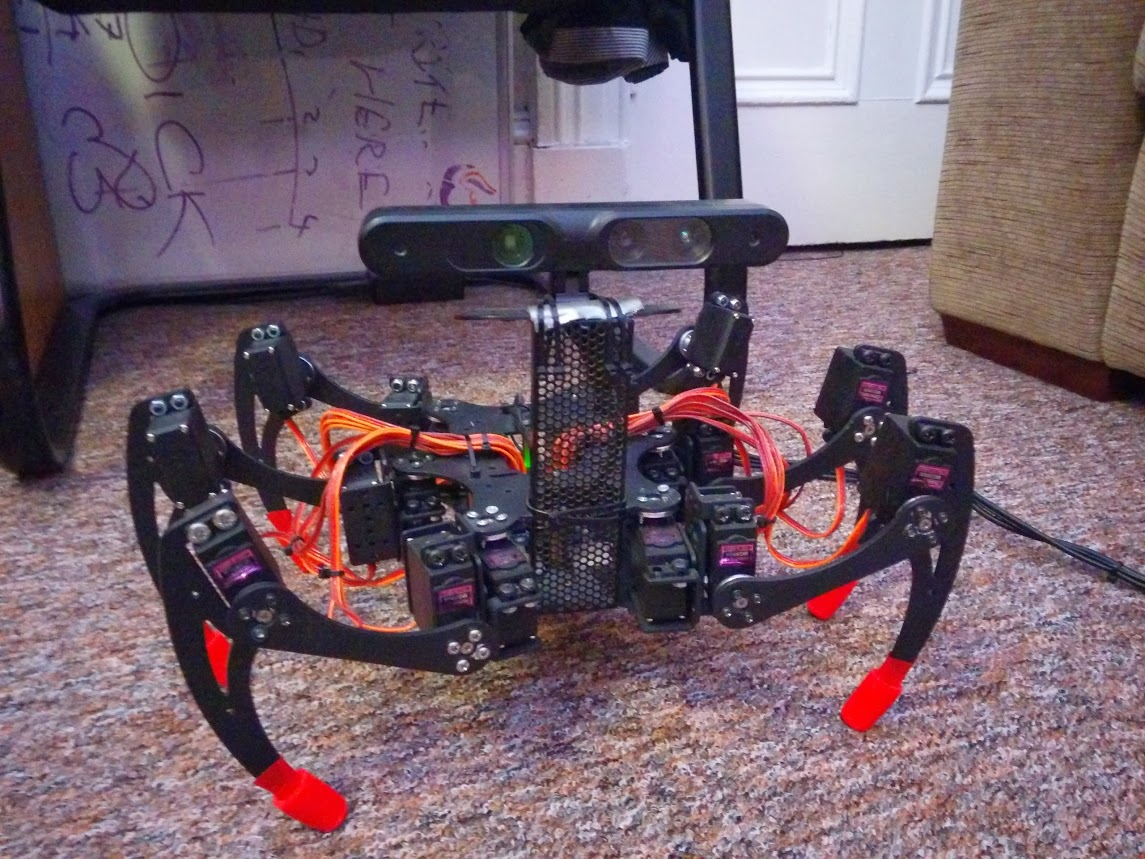
\includegraphics[width=10cm]{hexapod_body1}
    \caption{This hexapod-type robot which is used as the target hardware platform for this project. The robot has six limbs with three actuators on each, for a total of eighteen actuators. A RGB-D camera sits atop as the primary sensor, providing the robot with a 3D view of its immediate environment. A controller sits within the base of the robot, providing the necessary signals to operate the actuators. A bundle of cables protrudes from the back connecting the hardware to a nearby computer for operation, as well as a power source.}
    \label{fig:hexapod}
\end{figure}

This report will detail how this objective was achieved with great success. Through the use of ROS and its packages, it was possible to implement a control system that provides a number of these complex behaviours with relative brevity and simplicity. The resulting robot control system has a number of impressive capabilities:

\begin{description}
	\item[Hardware Operations] \hfill \\
	The system is capable with interacting with the RGB-D camera and servo controller on-board the robot. Commands can be sent through the system to the controller, allowing for the movement of any particular actuator. Image data from the sensor is received, processed, and then broadcast throughout the system, such that any subsystem needing the imagery can access it.

	\item[Locomotion] \hfill \\
	The system allows the robot to walk with a tripod-type walk gait in an abstracted manner. This abstraction allows any control subsystems to request linear and angular movements, without regard as to the specific actuator commands. The system also provides a means for calibrating the actuators, allowing for movements to be made precisely. Additionally, the robot can be manually controlled via a standard game controller.

	\item[Sensing] \hfill \\
	The system is capable of building a 3D map of the environment around the robot, updating in real-time as the robot moves around. This map is stored in an efficient manner, allowing the system to quickly determine if any obstacles are nearby. Additionally, the system is capable of localising the position of the robot relative its environment.

	\item[Navigation] \hfill \\
	The system is capable of fully autonomous navigation. Given a target position, the system will determine the most efficient path through the known environment and then supply the appropriate commands to move the robot to that position. Should the robot encounter any new obstacles, the path will be recalculated in real-time to avoid that obstacle.

\end{description}

Without access to the packages available for use through ROS, each of these capabilities would have taken a great number of person hours to develop, test and integrate. 

\section{Motivation}

The primary motivation was to show that it is possible to implement these complex behaviours, previously restricted to research projects with large budgets, on robots utilising cheaper consumer components. Laser range-finders, in particular, are typically used for environment scanning and positional tracking. These scanners provide extremely accurate results but can cost multiple thousands of pounds. However, as RGB-D sensors become increasingly available, it is possible to achieve similar results at a fraction of the cost with reduced accuracy.

As a secondary motivation, we wanted to show that it was possible to implement these behaviours without having to invest an immense number of person hours. Through the use of readily available libraries and frameworks, it is possible for a very small team to implement these behaviours without having to fully understand the underlying intricacies of any one system. Robot control systems are, simply, software development projects. By applying standard software development concepts, such as code reuse and separations of concerns, it allows us to make use of any existing works without having to "re-invent the wheel" each time.

Additionally, these behaviours, such as being able to move around and understand an environment, act as a general foundation for any further developments. The ramifications of being able to rapidly develop these robot system are such that new developments and innovations can be made more quickly, with less overall cost in terms of both budget and time.

\section{Overview}

To give further context to the project, we provide the following overview of the control system. The control system is divided into a number of subsystems, each dealing with a particular task necessary for achieving the behaviours described in the opening text. Each subsystem is additionally divided into more discrete nodes, as discussed in the later sections. These subsystems are referred to throughout the report and are described briefly below.

\begin{description}
	\item[Hardware Operations] \hfill \\
	This subsystem provides the necessary drivers to communicate with the robot hardware, converting any device-specific data into more generic formats that can be used elsewhere in the system.

	\item[Locomotion] \hfill \\
	This subsystem provides the robot with a means of moving itself around the environment in an abstracted manner, hiding the complexities of any actuator control.

	\item[Sensing] \hfill \\
	This subsystem interprets sensory data in a meaningful way, building up a view of the environment around the robot.

	\item[Navigation] \hfill \\
	This subsystem combines the sensing and locomotion subsystems to achieve autonomous navigation through the environment surrounding the robot.
\end{description}

ROS is used as a framework for implementing this control system, providing a means of communication between each component. Where possible, built-in and community-provided ROS packages are used to provide the implementation, rather than relying on any self-sourced code. A high-level overview of the system is shown in \autoref{fig:overview}, showing the connectivity between each subsystem and the underlying hardware it relies on. Upon starting the system, each subsystem begins communicating such that the complex behaviours can be performed by relying on data from one another.

\begin{figure}[h]
	\centering
	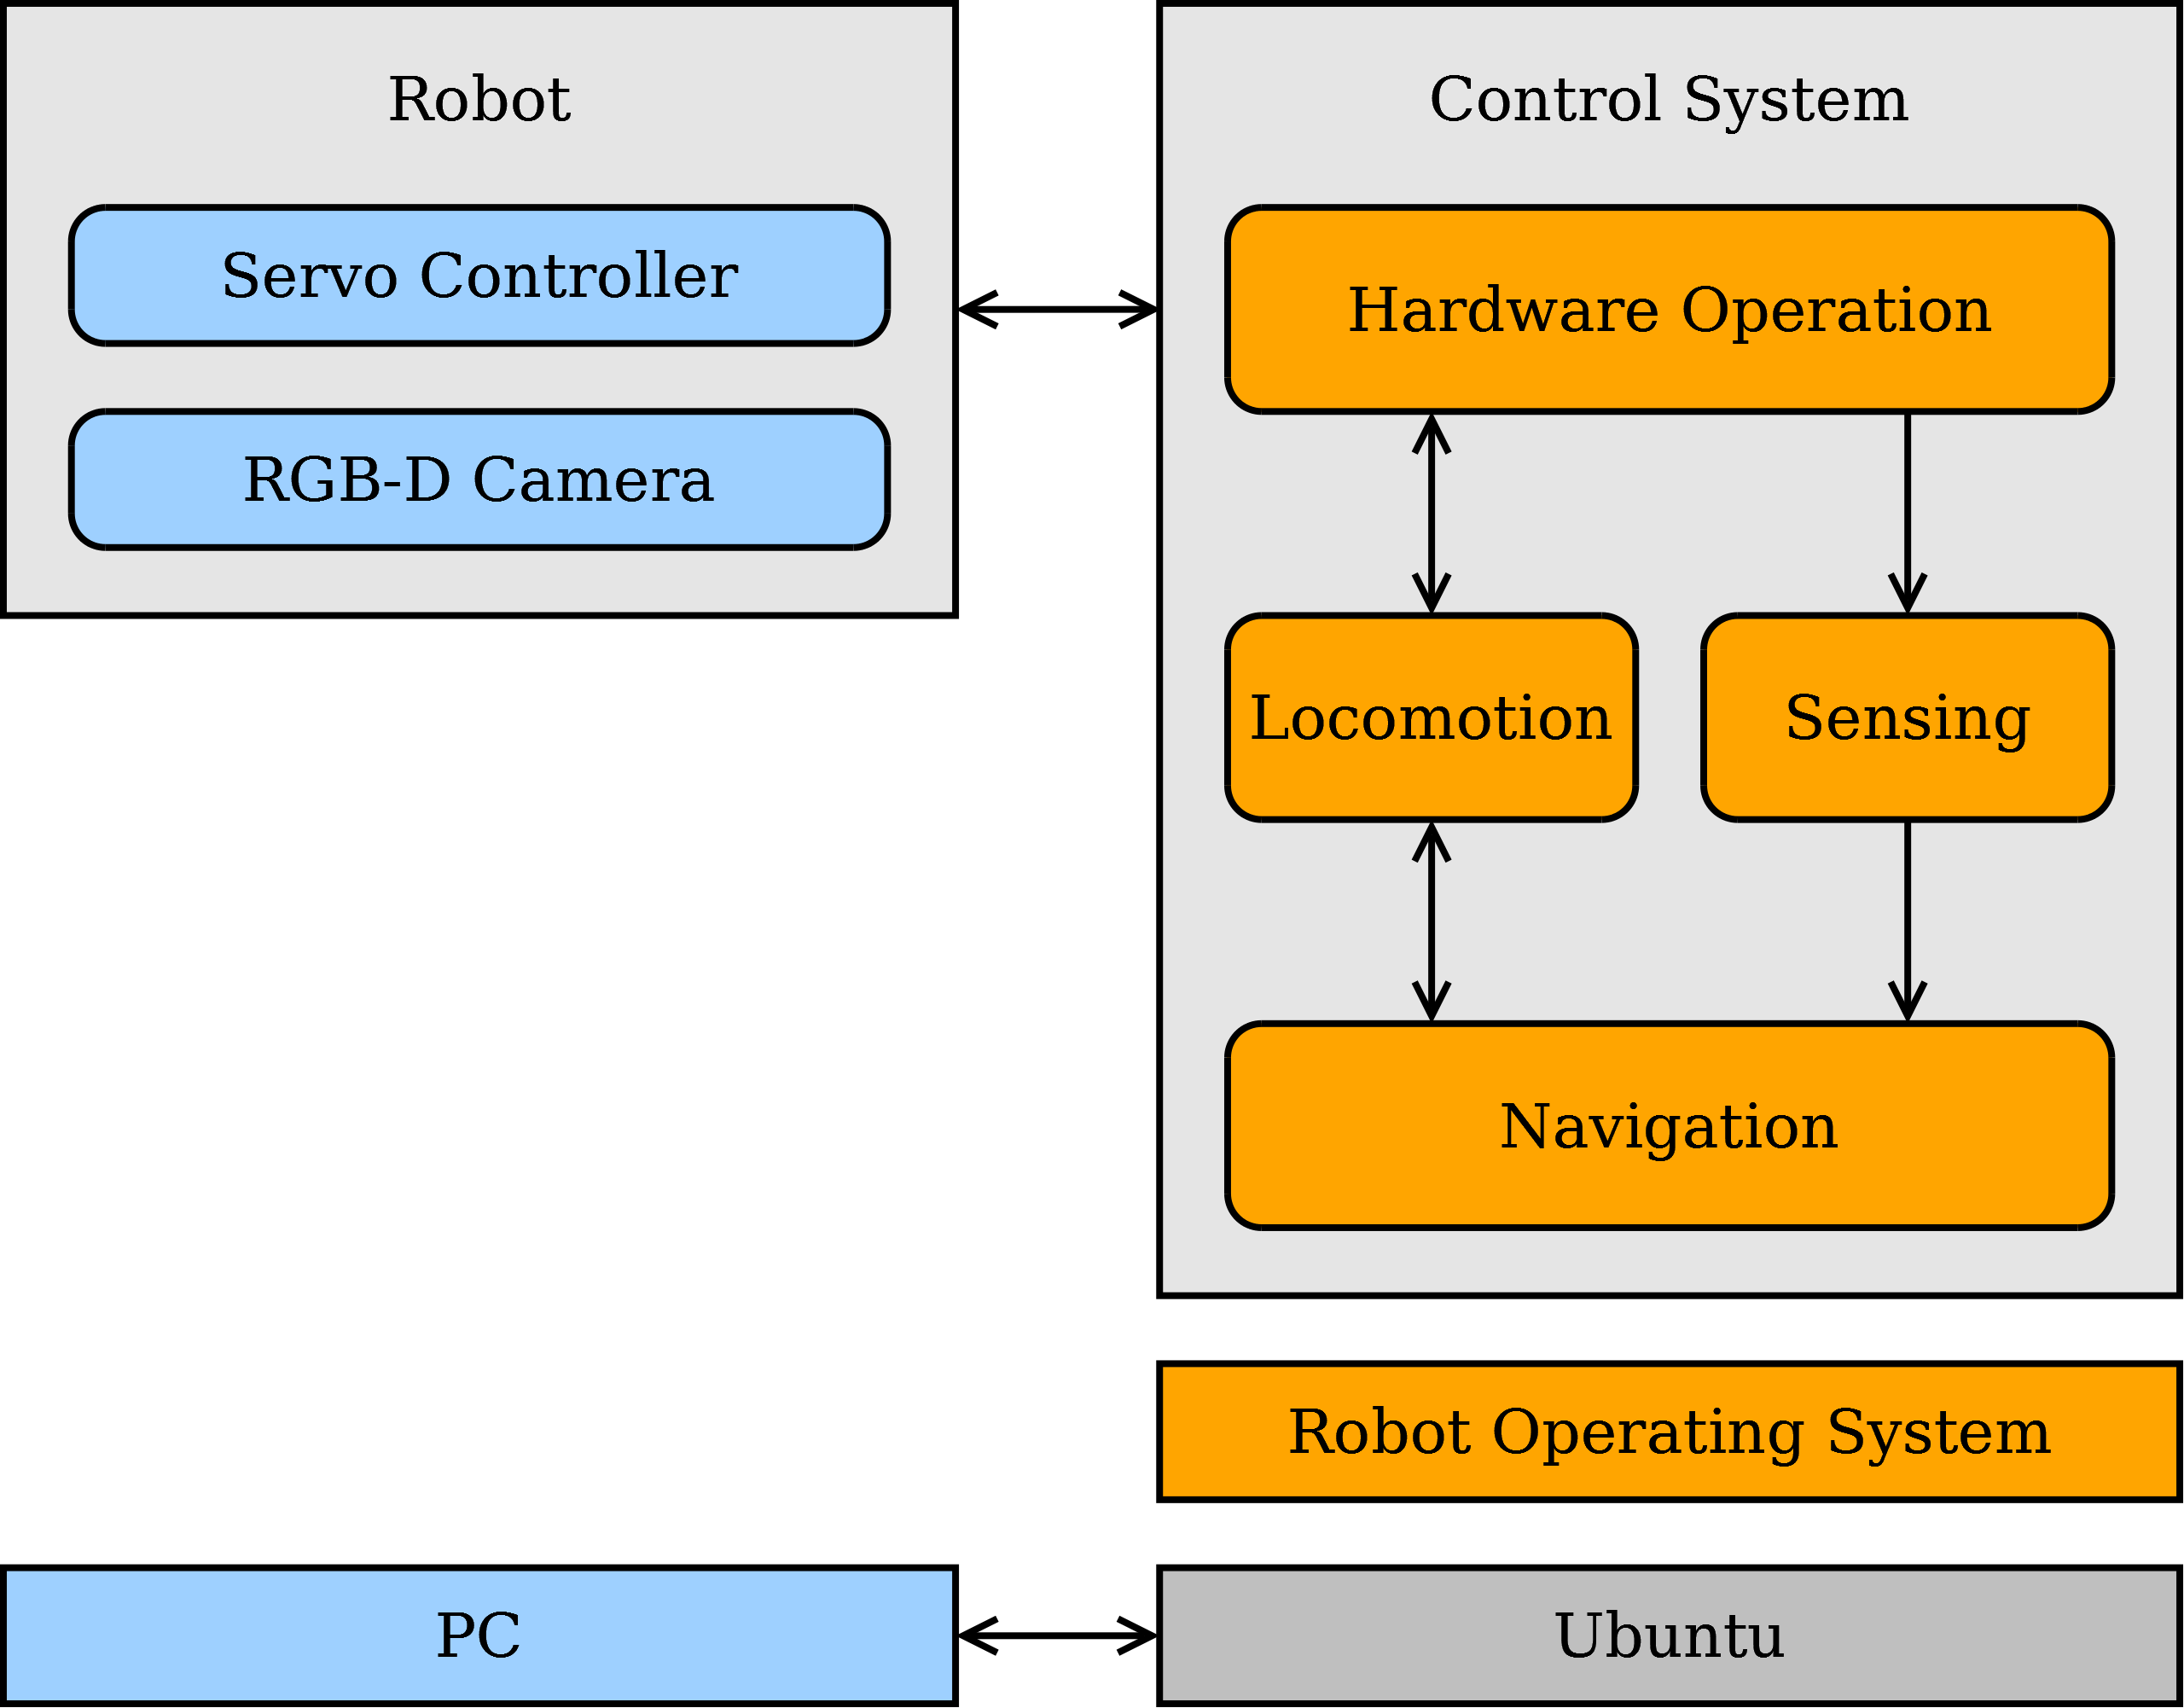
\includegraphics[width=10cm]{overview.png}
	\caption{This block diagram shows a high-level view of the robot control system. Arrows represent the communication channels between the different subsystems and hardware. Notably, communication between the hardware operation, sensing, and navigation subsystems is unidirectional only, as there is no sensor control available.}
	\label{fig:overview}
\end{figure}

As with any good software development project, this separation of concerns is essential for building a manageable system. The methods with which each subsystem communicate is generic, such that one can be replaced in its entirety with some other implementation, as long as it uses a similar interface. This also means that the subsystems can be used in other projects, should they be relevant.

\section{Outline}

The remainder of this report is divided into the chapters described below.

\begin{description}
	\item[Chapter~\ref{chap:background}: Background] \hfill \\
	This chapter elaborates on the context of the project, specifically the technical intricacies of ROS and the robot hardware. A number of existing robot systems will also be presented for comparison.

	\item[Chapter~\ref{chap:approach}: Approach] \hfill \\
	This chapter details the development approach used throughout the project, including the requirements for the robot control system.

	\item[Chapter~\ref{chap:implementation}: Implementation] \hfill \\
	This chapter explains the resulting implementation of the robot control system, elaborating on any design decisions or caveats.

	\item[Chapter~\ref{chap:evaluation}: Evaluation] \hfill \\
	This chapter presents the results on an evaluation of the performance of the robot control system, as well as detailing the experimental setup.

	\item[Chapter~\ref{chap:usage}: Usage] \hfill \\
	This chapter shows how the implemented robot control system is used. Specifically, how a user can interact with the control system, allowing navigational commands to be given.

	\item[Chapter~\ref{chap:conclusion}: Conclusion] \hfill \\
	This chapter summarises the report, providing a number of ideas for future development of the project.
\end{description}